%--------------------------------------------------------------
% Template author: Ben Montgomery
% Current revision: 1/23/2017
%--------------------------------------------------------------

\documentclass[12pt]{article}
\usepackage{amsmath} 
\usepackage{adjustbox}
\usepackage[margin=1in]{geometry} 
\usepackage{amsthm, listings, amssymb}
\usepackage{float, mathtools}
\usepackage{breqn}
\usepackage{array,multirow,graphicx}

 % ----------New special chars of computer scientists----------
\DeclarePairedDelimiter\ceil{\lceil}{\rceil}
\DeclarePairedDelimiter\floor{\lfloor}{\rfloor} 
\newcommand{\N}{\mathbb{N}}
\newcommand{\R}{\mathbb{R}}
\newcommand{\Z}{\mathbb{Z}}
 
 % --------------New problem-solving enviroments--------------
\newenvironment{exercise}[2][Exercise]{\begin{trivlist}
\item[\hskip \labelsep {\bfseries #1}\hskip \labelsep {\bfseries #2.}]}{\end{trivlist}}
\newenvironment{problem}[2][Problem]{\begin{trivlist}
\item[\hskip \labelsep {\bfseries #1}\hskip \labelsep {\bfseries #2.}]}{\end{trivlist}}

\newenvironment{solution}{\begin{proof}[Solution]}{\end{proof}}

% --------------------------------------------------------------
\begin{document}
\title{Program 1 --- COS 485}
\author{Samuel Barton \and Ben Montgomery \and Tyler Nelson}
\date{May 1, 2017}
 
\maketitle
\section{Algorithm Overview}

To get our base solution
we iteratively run Dikjstra's shortest paths algorithm starting from each of the
target nodes, and take the shortest overall that leads from our starting node to
another target node. We then set the cost of this path to zero. Repeat until we
have connected all target nodes in a non-cyclic manner.
\\
\\
With this base solution, we then run an iterative improvement algorithm which 
forbids the use of any edges in the current solution, and then reruns the base
algorithm. If we improve the cost, then keep the new solution. Repeat until
we no longer improve our solution.

\section{Algorithm Analysis}

Let us define a system of costs and variables as the following:
\begin{enumerate}
    \item Let us assign a cost of $1$ to basic mathematical operations, individual Boolean statements, if statements, array accesses, and variable assignments.
    \item Let datastructure (Arrays, HashMaps, Priority Queues...) initialization have a cost equal to the number of elements it is initially given the capacity for.
    \item Let us have $t$ target nodes in the Steiner tree.
    \item Let us have $v$ vertices in the graph.
    \item Let us have $e$ edges in the graph.
    \item Let a selected shortest path from Dijkstra's Shortest Paths algorithm have a length of $d$.
\end{enumerate}

Below we analyze the runtime of each method used in our solution. Further 
discussion will follow.

\textbf{steinerTree:}
\begin{flalign*}
    1 + pathFinder + 1
\end{flalign*}

Reduces to
\begin{dmath*}
2v^4t - 2v^4 + 14v^3t - 6v^3 + 3v^2\lg(v - 1) + 7v^2t + 14v^2 + 7vt + 
2vt\lg(t - 1) - 2v\lg(t - 1) 
 + 5dv + 14v + 10e + t + 6  
\\
+
\\
4v^2 + 6v + 9 + 16e
\\
+
\\
\lambda
\left[
2 + 2v^4t^2 - 4v^4t + 6v^4 - 2v^3t^3 + 4v^3t^2 -19v^3t + 6v^2t^2 + 11v^3 + 
3v^2t\lg(v - 1) - 3v^2\lg(v - 1) + 7v^2t + 2vt^2\lg(t - 1) - 11vt^2 + 
3vt\lg(t - 1) + 3vt^2\lg(v - 1) + 4vt\lg(t - 1) + 8tv + 2v\lg(t - 1) - 7t^3 -
2t^3\lg(t - 1) + 5v + 4t^2\lg(t - 1) - 2t\lg(t - 1) - 5t + 7e
\right] + 6e + 2
\end{dmath*}
\textbf{pathFinder (Base Solution):}
\begin{flalign*}
    2 + t + 2 + 4e + v + 4v + v(getShortestPath + 5d) + 1 + 6v + 1 + 6e
\end{flalign*}

Reduces to
\begin{dmath*}
2v^4t - 2v^4 + 14v^3t - 6v^3 + 3v^2\lg(v - 1) + 7v^2t + 14v^2 + 7vt + 
2vt\lg(t - 1) - 2v\lg(t - 1) 
 + 5dv + 14v + 10e + t + 6  
\end{dmath*}
\textbf{pathFinder (Iterative Improvement Setup):}
\begin{flalign*}
    2v + 4 + updateNumberOfConnections + 2 + 4e + 2e + 1 + 4e + 6e 
\end{flalign*}

Reduces to
$$
    4v^2 + 6v + 9 + 16e
$$
We must pause to recognize that in theory, the iterative improvement could run for an 
exceedingly long amount of time. The probability of this happening is incredibly slim,
and can be demonstrated by the Monte Carlo method; however, it is worth recognizing 
that in the worst case, this program could spend its time improving its solution by
some number bounded by $\lambda = e^e$.
\\
\\
\textbf{pathFinder (Iterative Improvement):}
\begin{dmath*}
    \lambda 
        \left\{
            2 +\\
            (v - t)
            \left[ 
                5 + 
                3(v - 1) + 
                3 + 
                (t - 1)
                \left(
                    1 + 
                    getShortestPath +
                    1 +
                    getPath +
                    3 (v - 1) 
                \right) \\+
                2 +
                7e +
                2 +
                v +
                \left(
                    2 + 
                    4(v - 1) +
                    3
                \right) \\ + 
                v (2 + 1 + betterTrimmer) +
                3 +
                \left(
                    2 + v  +
                    4(v-1) 
                \right)
            \right] 
        \right\} + 6e
\end{dmath*}

Reduces to
\begin{dmath*}
\lambda
\left[
2 + 2v^4t^2 - 4v^4t + 6v^4 - 2v^3t^3 + 4v^3t^2 -19v^3t + 6v^2t^2 + 11v^3 + 
3v^2t\lg(v - 1) - 3v^2\lg(v - 1) + 7v^2t + 2vt^2\lg(t - 1) - 11vt^2 + 
3vt\lg(t - 1) + 3vt^2\lg(v - 1) + 4vt\lg(t - 1) + 8tv + 2v\lg(t - 1) - 7t^3 -
2t^3\lg(t - 1) + 5v + 4t^2\lg(t - 1) - 2t\lg(t - 1) - 5t + 7e
\right] + 6e
\end{dmath*}

\textbf{getShortestPath:}
\begin{dmath*}
    1 + shortestPaths + 1 + 
    (6v + (t-1))
    + (t - 1) \lg (t - 1) + 1\\
    + (t-1)(7 + hasCycle + replacePath) + 1 + (t - 1) \lg (t - 1) + 2
\end{dmath*}
Reduces to
$$
2v^3t - 2v^3 + 14v^2t - 6v^2 + 3v\lg(v - 1) + 7vt + 14v + 7t + 2t\lg(t - 1) -
2\lg(t - 1) + 3
$$

\textbf{getPath:}
\begin{dmath*}
3 + 
(v - 1)
\left[
    3 + 5(v - 1) + 1
\right]
\end{dmath*}

Reduces to
$$
5v^2 - 6v + 4
$$

\textbf{hasCycle:}
\begin{dmath*}
1 + innerHasCycle + 1 + 3v
\end{dmath*}

Reduces to
$$
2v^3 - 13v^2 + 15v + 2
$$

\textbf{innerHasCycle:}
\begin{dmath*}
v
\left[1 + (v - 1)
    \left(
        2 + vertexInPath + 11
    \right)
\right]
\end{dmath*}

Reduces to
$$
2v^3 - 13v^2 + 12v
$$
\textbf{vertexInPath:}
\begin{dmath*}
2(v - 1)
\end{dmath*}

Reduces to
$$
2v - 2
$$
\textbf{replacePath:}
\begin{dmath*}
2 + (v - 1)
\left[
    3 + 5(v - 1) + 7
\right]
\end{dmath*}

Reduces to
$$
5v^2 - 3
$$
\textbf{zeroPath:}
\begin{dmath*}
2 + 
(v - 1)
\left[
    3 + 6(v - 1)
\right]
\end{dmath*}

Reduces to
$$
6v^2 - 9v + 5
$$
\textbf{betterTrimmer:}
\begin{dmath*}
(v - 1)
\left[
    8 + 2(v - 1) + 8
\right] 
\end{dmath*}

Reduces to
$$
2v^2 + 12v - 14
$$
\textbf{shortestPaths:}
\begin{dmath*}
5 + v
\left[
    6 + 8(v - 1) + 3 + 3\lg(v - 1)
\right]
\end{dmath*}

Reduces to
$$
8v^2 + 3v\lg(v - 1) + v + 5
$$
%
\textbf{updateNumberOfConnections:}
\begin{dmath*}
2 + v
\left[
3 + 4(v - 1) + 5
\right]
\end{dmath*}

Reduces to
$$
4v^2 + 4v + 2
$$

\subsection*{Further Discussion}

After digesting the gratuitous complexity of the preceeding page and a half of
insanity we assure the reader that the base solution, as analyzed in the 
piece entitled \textbf{pathFinder (Base Solution):}, provides answers to within
the 10\% bound of the ``optimal'' provided solutions in time 
$$
T_n \in \Theta(v^4t)
$$
Now, we may choose to employ an iterative improvement optimization algorithm to 
our current solution. The runtime for this piece is analyzed in the section
\textbf{pathFinder (Iterative Improvement):} and will have time
$$
T_n \in \Theta(\lambda(v^4t^2))
$$
where $\lambda$ is a bound which could possibly be at worst $e^e$. This would 
happen if every time reevaluated our standing solution, then we found an
improvement to make, and this improvement used 1 edge that was not used before;
however, now that we have made that new connection, we can remake any prior 
connection that we had before. This means that in the worst case, every edge
will effectively be able to look at any possible solution to the problem.

\section{Program Output}

\subsection*{Results Tab}

\begin{figure}[h]
    \centering
    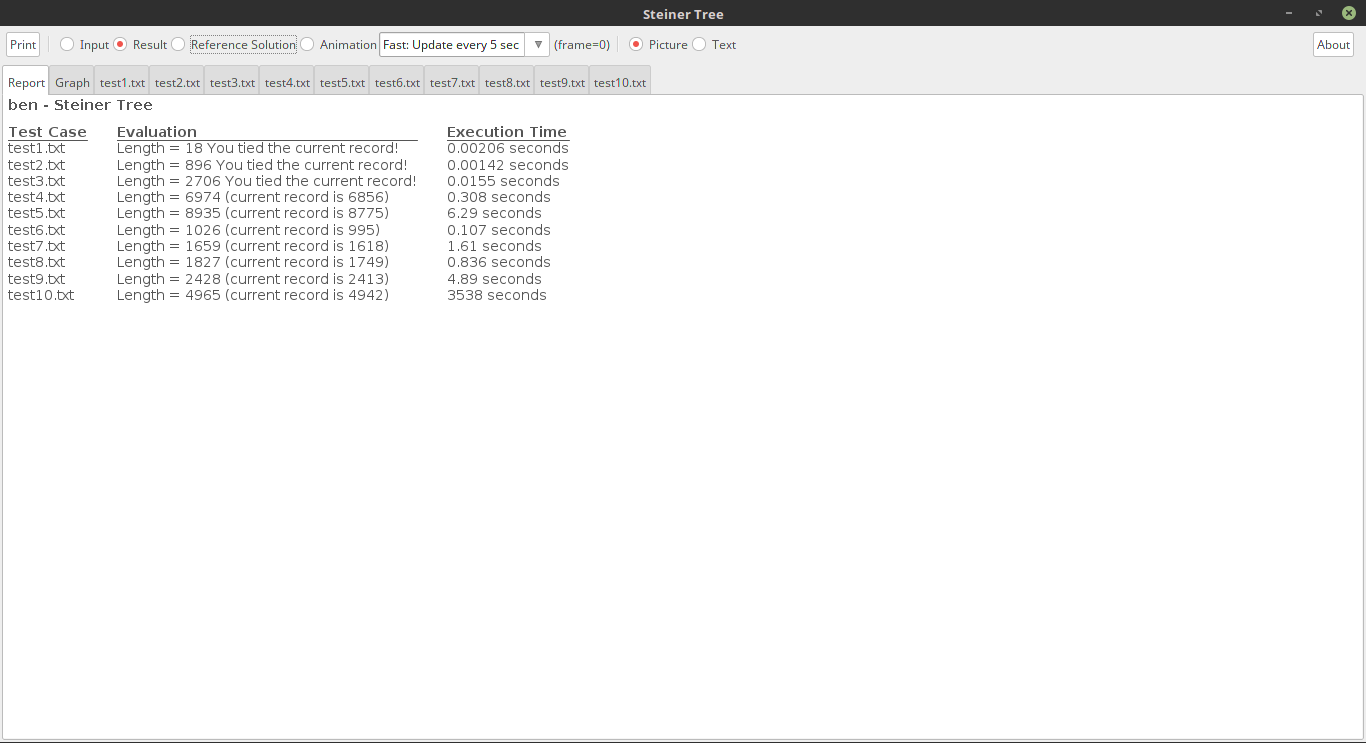
\includegraphics[width=0.75\textwidth]{restab.png}
\end{figure}
\newpage
\subsection*{Test 4 Output}

\begin{figure}[h]
    \centering
    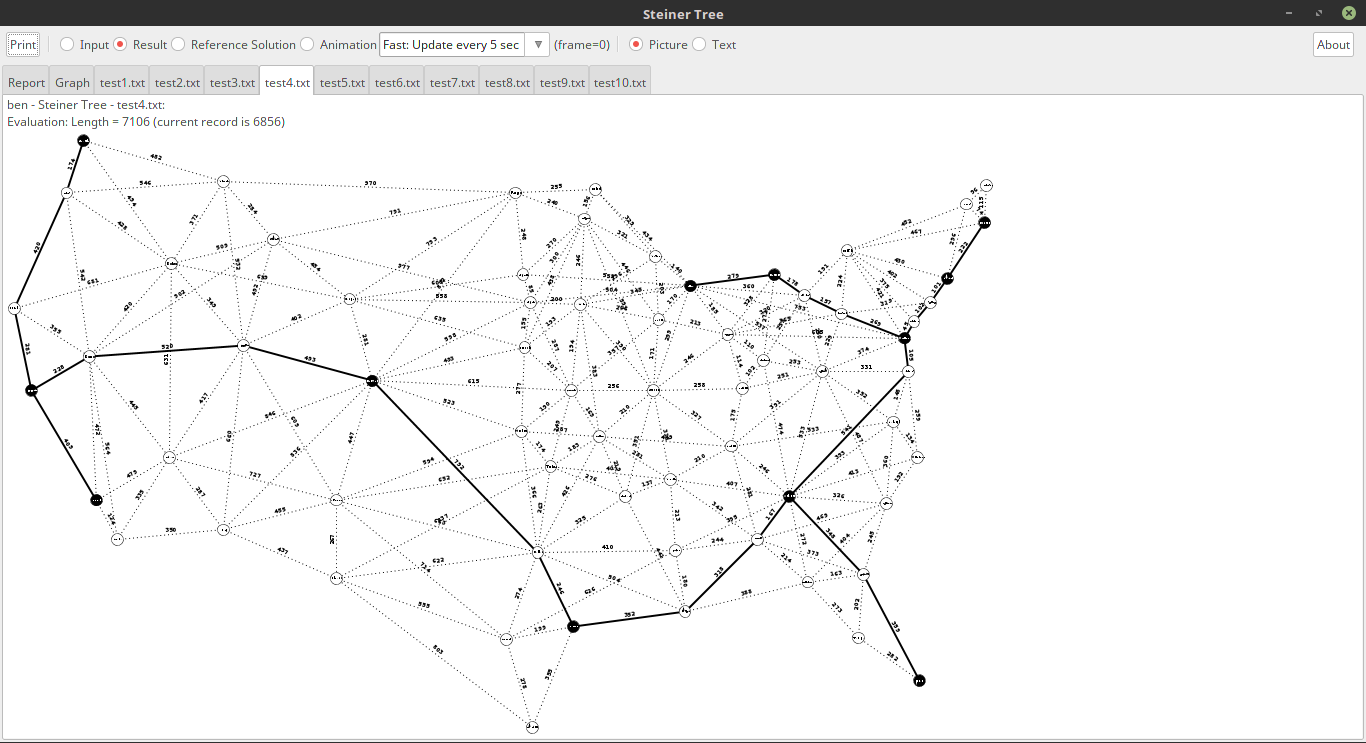
\includegraphics[width=0.75\textwidth]{test4.png}
\end{figure}

\section{Code Listing}
\subsection*{SteinerTree.java}
\lstset{basicstyle=\ttfamily\scriptsize, language=java}
\lstinputlisting[language=java]{SteinerTree.java}
\pagebreak
\subsection*{WeightedVertex.java}
\lstinputlisting[language=java]{WeightedVertex.java}

\end{document}
